% \begin{frame}{Recursos}
%     \begin{figure}
%         \centering
%         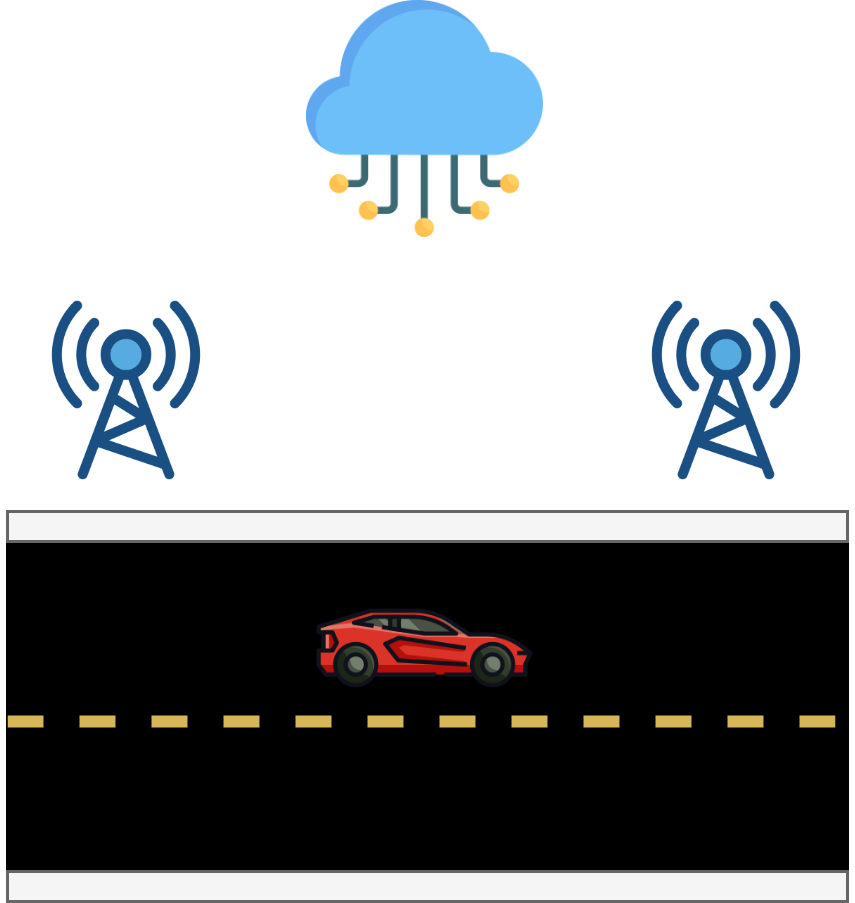
\includegraphics[width=0.7\textwidth]{Figuras/cav-scenario.png}
%     \end{figure}
% \end{frame}

% \begin{frame}{Tarefas}
%     \begin{figure}
%         \centering
%         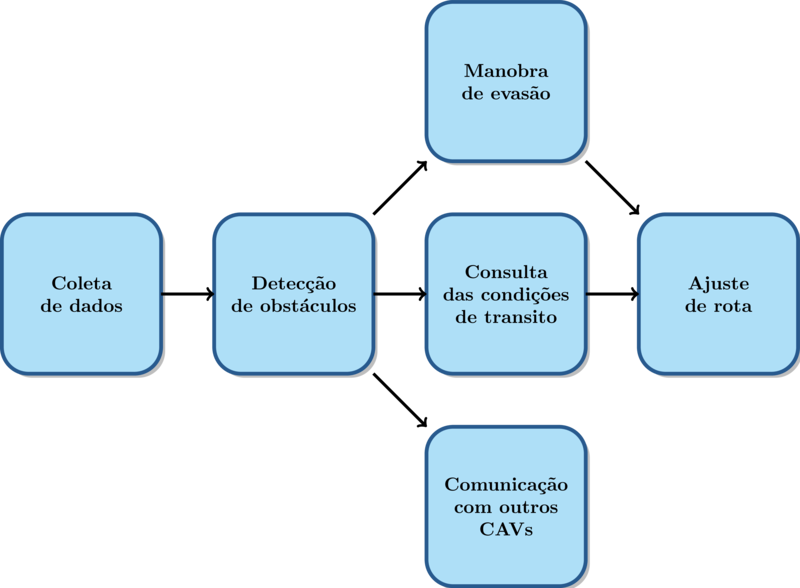
\includegraphics[width=0.8\textwidth]{Figuras/cav-task.png}
%     \end{figure}
% \end{frame}

\begin{frame}{Escalonamento}
    \begin{figure}
        \centering
        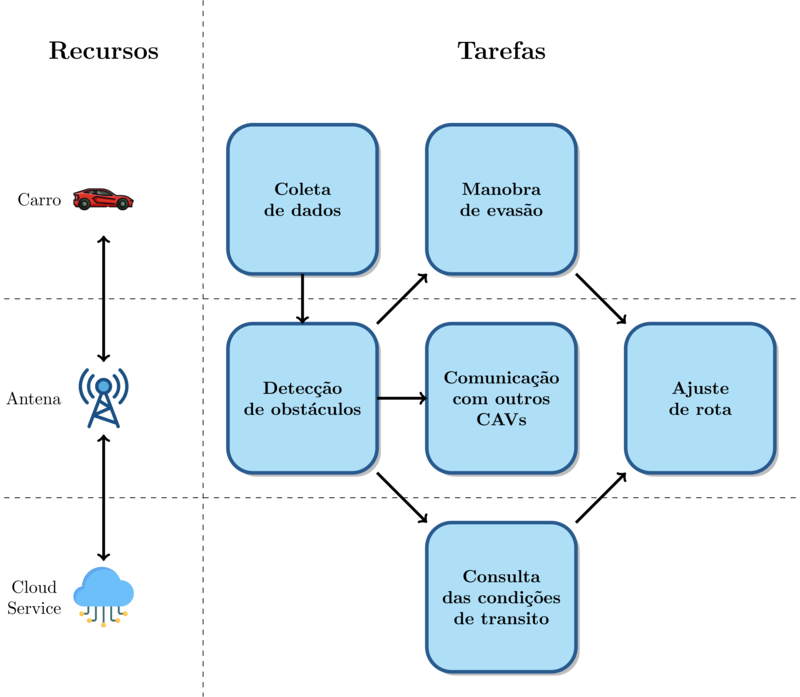
\includegraphics[width=0.8\textwidth]{Figuras/cav-scheduling.png}
    \end{figure}
\end{frame}

\begin{frame}{Escalonamento de Recursos}
    Problema conhecido na literatura.
    \begin{itemize}
        \item NP-Hard.
        \item Diversidade de soluções propostas.
        \begin{itemize}
            \item[--] ADMM, Heft, Page Rank, Polaris, etc.
        \end{itemize}
    \end{itemize}
\end{frame}

\begin{frame}{Escalonamento de Recursos}
    Dificuldades encontradas ao desenvolver algoritmos de escalonamento em Edge-Cloud Continuum:
    \begin{itemize}
        \item Modelagem do problema não padronizada.
        \item Código fechado.
        \item Falta de componentes comuns de alto desempenho.
    \end{itemize}
\end{frame}

\begin{frame}{Escalonamento de Recursos}
    Solução:

    Framework
    \begin{itemize}
        \item[] de código aberto
        \item[] que incorpora componentes comuns a algoritmos de escalonamento
        \item[] focado em alto desempenho.
    \end{itemize}
\end{frame}